\documentclass[12pt]{article}

\usepackage{ctex}
\usepackage{float}
%\setlength{\baselineskip}{20pt}
\usepackage[bottom=2.5cm,top=2.5cm,left=2.5cm,right=2cm]{geometry}
\usepackage{graphicx}
\usepackage{amsmath}
\usepackage{caption}
\usepackage{subcaption}
\usepackage{cite}

\title{\heiti 矩阵乘积态与含时变分原理}
\author{\kaishu 吴继宏 }
\date{\today}
\usepackage{fancyhdr}
\pagestyle{fancy}
\fancyhf{}
\fancyhead[R]{\songti 矩阵乘积态与含时变分原理}
\fancyhead[L]{\songti 兰州大学本科毕业论文(设计)}
\fancyfoot[C]{\songti\thepage}



\begin{document}
	
	\maketitle

	\newpage
	{\centering\tableofcontents}
	\newpage
	{\centering\textbf{矩阵乘积态与含时变分原理}}\\
	{\centering\section*{摘要}}
	量子多体系统是凝聚态物理领域研究的核心问题,然而无论是解析求解还是数值模拟,这些系统都很难研究,原因是多体系统的希尔伯特空间维度随系统粒子数的增加而指数增加。最近二十年随着张量网络算法的研究,人们得以对于量子系统中最重要的性质——关联和纠缠深入理解。本文首先简单讲解了张量的基础知识以及基于SVD分解描述一维量子系统的矩阵乘积态,然后详细地介绍了目前主要的几种基于矩阵乘积态研究的张量网络算法,最后利用这些算法对一些可解的量子系统(一维横场伊辛模型和一维XXZ模型)进行模拟,求解其基态相关性质以及淬火之后的动力学行为,并与解析结果比较。对于这些简单系统的研究,可以帮助我们更好的理解量子多体系统的性质,包括纠缠和热化等。\\~\\
	{\heiti 关键词:}张量网络算法; 矩阵乘积态; 含时变分原理; 一维横场伊辛模型; 关联函数;
	
	\newpage
	{\centering \textbf{Matrix Product State and Time-denpendent Variational Principle}}
	{\centering\section*{Abstract}}
	Quantum many body systems is a key problem in condensed matter theory, however, it is very hard to analyze no matter in theoretical derivation or numerical simulation. The main reason is that the dimension of Hilbert space is exponential to the number of particles. With the development of tensor network algorithm, researcher could get deeper understanding of correlation and entanglement, which are the most important features of quantum systems. In the organization of this people, it first gives a simple introduction of tensor and matrix product state using SVD, then discusses several mainstream algorithms based on MPS. At last, I use these algorithms to simulate TFIM and XXZ model, analyzing properties of ground states and quench dynamics, comparing with theoretical equations. Research on these simple quantum systems, we can better understand features of quantum many body systems, including entanglement and thermalization.\\~\\
	\textbf{Keyword:} Tensor network algorithm;Matrix product state;Time dependent variational principle;TFIM;correlation function
	

	\newpage
	{\centering\section{引言}}
	量子多体系统中的涨落和关联作用可以引出许多有趣的现象,著名的例子比如量子分数霍尔效应,自旋液体和高温超导等。理解这些多体系统中的涌现性质是一个非常重要且极具挑战的问题。最主要的问题是多体系统的希尔伯特空间随微观状态数呈指数增长,也就是所谓的“指数墙”问题:描述n体量子系统的参数是随着n呈指数增长,超出了如今计算机的计算性能。当然也有一些方法研究一些特定的量子多体问题,例如一些完全可解的量子系统以及量子蒙特卡罗模拟,但是量子蒙特卡罗模拟在一些系统会出现符号问题而失效。因此以张量乘积态为基础的算法在量子多体系统的模拟上显示出了极强的有效性。
	
	1992年White提出了密度矩阵重整化群算法(Density Matrix Renormalization Group, DMRG),成为了研究一维量子格点系统强大的数值方法。另一方面,矩阵乘积态(Matrix Product State)作为量子态的描述用于一维AKLT态的研究。随后DMRG和MPS相融合,建立了一套新的DMRG算法机制,通过变分优化MPS的方法,得到系统的基态。随后相关的算法不断涌现,迅速成为研究量子多体模型最强大的数值方法之一。DMRG的成功之处还在于它可以用来模拟实时演化去研究系统的输运和非平衡性质,但是系统波函数的两体纠缠熵会随着时间迅速增加,将导致巨大的计算成本。
	
	利用这些数值方法,我们可以研究多体系统的非平衡问题。通常当我们研究一个系统的性质时,我们忽略了其微观细节简化对于复杂系统的分析,建立起重要并普遍的原理。目前普遍认为量子多体系统可以用随机矩阵理论(Random Matrix Theory)来描述——系统会演化到熵最大的热力学平衡态。但随着量子模拟的不断发展,研究者发现了一些不符合该理论描述的系统包括量子多体局域(Many Body Localization)以及量子多体疤痕(Many Body Scar)\cite{papic2021weak}。因此张量网络相关的数值算法,能为我们对于这些系统的研究提供有效的支持和帮助。
	\newpage
	

	{\centering\section{矩阵乘积态}}
	   \subsection{张量基础知识}
	   在介绍矩阵乘积态之前,先简单介绍一下张量。常见的向量和矩阵分别对应于一阶张量和二阶张量,为了在张量网络中方便的表示出更高阶张量,我们采用如下图中的图形表示来更方便的描述张量。
	   \begin{figure}[H]
	   	\centering
	   	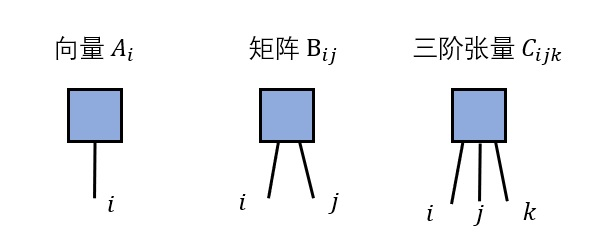
\includegraphics[scale=0.7]{1.张量图形表示}
	   	\caption[10.5pt]{ 张量图形表示}
	   	\label{fig:1}
	   \end{figure}
   
	   利用该图形表示,可以方便的表示出张量网络的收缩方式,如$ D_{ijk}=\sum_{lmn}A_{ilm}B_{ijn}C_{nmk} $ 三阶张量$ D_{ijk}$由三个三阶张量缩并形成,在图形表示中,两个张量相同的指标的缩并用相应“腿”相连形成。
	   \begin{figure}[H]
	   	\centering
	   	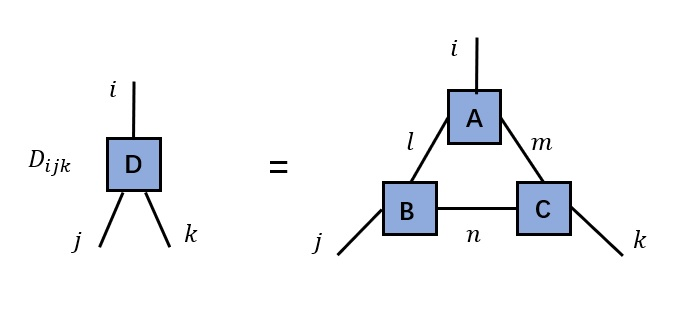
\includegraphics[scale=0.7]{2.张量网络收缩}
	   	\caption[9pt]{ 张量收缩}
	   	\label{fig:2}
	   \end{figure}
   
	   对于张量的指标还有另外两个操作:排列(permute)和重组(reshape)。排列即张量的元素个数保持不变,改变张量的不同指标的顺序,如矩阵的转置,交换了行指标和列指标的顺序。重组即保持张量的元素个数不变,将其中的某些指标合并为一个指标,如我们可以将一个$2\times3\times4$的三阶张量的前两个指标合并为一个维度为$6$的大指标,该张量变为一个$6\times4$的矩阵。
	   
	   有了上述关于张量的基本认识和相应操作,接下来就可以利用这些操作以及矩阵的正交分解(SVD分解,QR分解)得到矩阵乘积态的表示(Matrix product state)
	   
	   \subsection{矩阵乘积态表示}
	   我们考虑一个一维N格点的量子系统,整个系统的希尔伯特空间基矢是N个单粒子希尔伯特空间基矢的直积。用$|j_n\rangle$表示第n个单粒子基矢。总系统的一个任意的量子态$|\Psi\rangle$可以表示为\cite{schollwock2011density} $|\Psi\rangle=\sum_{j_1,...,j_N}C_{j_1,...,j_N}|j_1,...,j_N\rangle$。矩阵乘积态是将波函数系数$C_{j_1,...,j_N}$分解为一系列矩阵的乘积形式:
	   \begin{equation}\begin{split}
	   	|\Psi\rangle&=\sum_{j_1,...,j_N}\sum_{\alpha_2,...,\alpha_3}M_{\alpha_1\alpha_2}^{[1]j_1}...M_{\alpha_N\alpha_{N+1}}^{[N]j_N}|j_1,...,j_N\rangle\\ &=\sum_{j_1,...,j_N}M^{[1]j_1}...M^{[N]j_N}|j_1,...,j_N\rangle
	   \end{split}.\end{equation}
       我们将一个含有N指标的系数(N阶张量)$ C_{j_1,...,j_N} $变为了N个矩阵的乘积$ M^{[1]j_1}M^{[2]j_2}...M^{[N]j_N} $,其中每一个$M^{[n]j_n}$的维度为$ \chi_n\times\chi_{n+1} $,$\alpha_n$称为虚拟指标,$j_n$称为物理指标。两个边界的$M^{[1]j_1},M^{[N]j_N}$分别为行矢量和列矢量,这样整个矩阵乘积的结果就是一个数即$C_{j_1,...,j_N}$
       \begin{figure}[H]
       	\centering
       	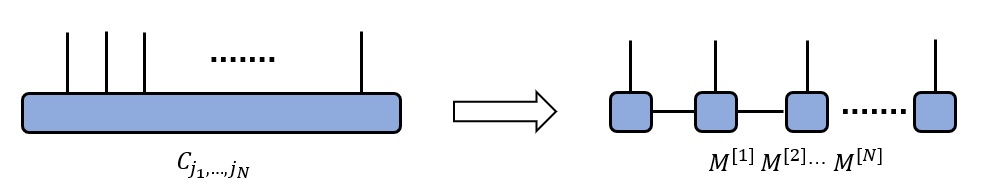
\includegraphics[scale=0.7]{3.矩阵乘积态示意}
       	\caption[9pt]{ 矩阵乘积态示意}
       	\label{fig:3}
       \end{figure}
       
       \subsubsection{SVD分解和Schmidt分解}
       奇异值分解(singular value decomposition)将任意的$N_A\times N_B$的矩阵M分解为:$$M=USV^{\dagger}$$其中U的维度为$(N_A\times min(N_A,N_B))$,并且是正交矩阵有$U^{\dagger}U=I$;S是维度为$min(N_A,N_B)\times min(N_A,N_B)$的对角矩阵;V的维度为$min(N_A,N_B)\times N_B$,同样为正交矩阵$V^{\dagger}V=I$。
       SVD分解有一个很重要的性质,对角矩阵S的元素奇异值$S_i$是迅速的减小。我们可以通过对奇异值的截断对矩阵M作最优化的维度截断,截断后的矩阵M'维度小于初始的矩阵M。
       
       SVD的一个应用是我们可以对一个量子态作施密特分解(Schmidt decomposition)。考虑一个由AB两个子系统构成的纯态, 
       \begin{equation}|\Psi \rangle=\sum_{ij}\Psi_{ij}|i\rangle_A|j\rangle_B.\end{equation}
       其中$\{|i\rangle_A\}$和$\{|j\rangle_B\}$是A和B中的一组正交基,维度分别为$N_A$和$N_B$。对$\Psi_{ij}$作SVD分解得到
       \begin{equation}\begin{split}|\Psi\rangle &=\sum_{ij}\sum_{\alpha=1}^{min(N_A,N_B)}U_{i\alpha}S_{\alpha\alpha}V^{\dagger}_{j\alpha}|i\rangle_A|j\rangle_B\\ &=\sum_{\alpha=1}^{min(N_A,N_B)}(\sum_i U_{ia}|i\rangle_A)S_\alpha(\sum_jV^{\dagger}_{j\alpha}|j\rangle)\\ &=\sum_{\alpha=1}^{min(N_A,N_B)}S_\alpha|\alpha\rangle_A|\alpha\rangle_B.\end{split}\end{equation}
       由于$U$和$V^\dagger$的正交性质,新基矢$\{|\alpha\rangle_A\}$和$\{|\alpha\rangle_B\}$依然是正交基矢。于是我们得到施密特分解形式
       \begin{equation}|\Psi\rangle=\sum_{\alpha=1}^rS_\alpha|\alpha\rangle_A|\alpha\rangle_B.\end{equation}
       如果$r=1$就是一个直积态,如果$r>1$就是纠缠态。
       
       \subsubsection{将任意量子态分解成MPS}
       考虑有L个格点,每个格点维度为d维的系统。一个量子态表示为$|\Psi\rangle=\sum_{j_1,...,j_N}C_{j1,...,jN}|j_1,...,j_N\rangle$。
       
       第一步,将有$d^L$个元素的L阶张量重组为$d\times d^{L-1}$的矩阵,\begin{equation}\Phi_{j_1,(j_2,...,j_L)}=C_{j_1,...,j_N}.\end{equation}
       对$\Phi$进行SVD分解
       \begin{equation}\Phi_{j_1,(j_2,...,j_L)}=\sum_{\alpha_1}U_{j_1,\alpha_1}S_{\alpha_1,\alpha_1}V^\dagger_{\alpha_1,(j_2,...,j_L)}\equiv\sum_{\alpha_1}U_{j_1,\alpha_1}C_{\alpha_1j_2,...,j_L}.\end{equation}
       将$U_{j_1,\alpha_1}$记为$M_{\alpha_1}^{j_1}$,将S和V合并为C,并继续将C重组为$r_1d\times d^{L-2}$的矩阵
       \begin{equation}\Phi_{(\alpha_1j_2),(j_3,...,j_L)}=C_{\alpha_1j_2,...,j_L}.\end{equation}
       继续对$\Phi$作SVD分解
       \begin{equation}\Phi_{(\alpha_1j_2),(j_3,...,j_L)}=\sum_{\alpha_2}U_{(\alpha_1j_2),\alpha_2}S_{\alpha_2,\alpha_2}V^{\dagger}_{\alpha_2,(j_3,...,j_L)}.\end{equation}
       将$U_{(\alpha_1j_2),\alpha_2}$记为$M_{\alpha_1,\alpha_2}^{j_2}$。将S和V继续重组为$r_2d\times d^{L-3}$的矩阵作SVD分解。最终将得到
       \begin{equation}C_{\alpha_1j_2,...,j_L}=\sum_{\alpha_1,...,\alpha_{L-1}}M_{\alpha_1}^{j_1}M_{\alpha_1,\alpha_2}^{j_2}...M_{\alpha_{L-1}}^{j_L}.\end{equation}
       一个任意的量子态以矩阵乘积态的形式表示了出来
       \begin{equation}\Psi=\sum_{j_1,...,j_L}M^{j_1}M^{j_2}...M^{j_L}|j_1,..,j_L\rangle.\end{equation}
       其直观图形表示为
       \begin{figure}[H]
       	\centering
       	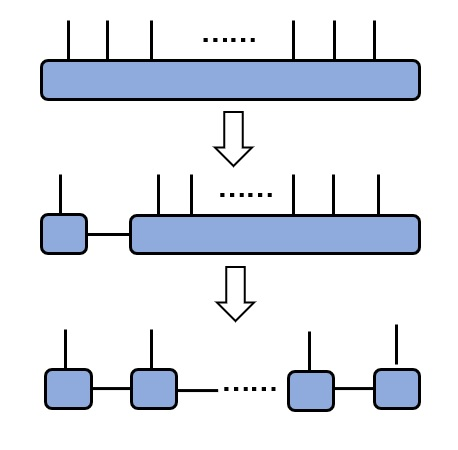
\includegraphics[scale=0.7]{4.矩阵乘积态分解}
       	\caption[9pt]{ 矩阵乘积态分解}
       	\label{fig:4}
       \end{figure}
       
        MPS表示一个好处是可以绕过“指数墙问题”,考虑N个格点,每个格点自由度为d,则需要$d^N$个参数完整来表示这个系统,这种指数增长远超目前计算机的计算规模。采取MPS表示时,我们可以在每一步SVD分解时规定最大的截断维度$\chi$来截取奇异值,这样只需要多项式增长的数据$Nd\chi^2$来描述多体系统。
        
        还有值得注意的一点是,除了上述的MPS表述外,矩阵乘积态也能用小维度的矩阵精确表示一些系统的状态。下面举例说明:
        
        考虑一维横场伊辛模型,其哈密顿量为
        \begin{equation}H=-\sum_n\sigma_n^z\sigma_{n+1}^z+g\sigma_n^x.\end{equation}
        当横场很强$g\gg1$时,系统的基态为$|\gets...\gets\rangle\equiv(\frac{1}{\sqrt{2}}|\uparrow\rangle-\frac{1}{\sqrt{2}}|\downarrow\rangle)\otimes...\otimes(\frac{1}{\sqrt{2}}|\uparrow\rangle-\frac{1}{\sqrt{2}}|\downarrow\rangle)$。用MPS表示该基态为
        \begin{equation}M^{[n]\uparrow}=\frac{1}{\sqrt{2}},\qquad M^{[n]\downarrow}=-\frac{1}{\sqrt{2}}.\end{equation}
        
        考虑Neel反铁磁态$|\uparrow\downarrow\uparrow\downarrow...\rangle$,我们用不同的矩阵表示奇偶格点,
        \begin{equation}M^{[2n-1]\uparrow}=M^{[2n]\downarrow}=1, \qquad M^{[2n-1]\downarrow}=M^{[2n]\uparrow}=0.\end{equation}
	   
	   \subsection{纠缠熵}
	   纠缠是量子力学中一个重要的现象,我们知道量子多体系统里的纠缠能帮助了解许多量子态的信息。根据上述的施密特分解,希尔伯特空间$H=H_A\otimes H_B$中的任意量子态可以表示为\cite{hauschild2018efficient}
	   \begin{equation}|\Psi\rangle=\sum_\alpha \Lambda_\alpha|\alpha\rangle_A\otimes|\alpha\rangle_B, \qquad |\alpha\rangle_{A(B)}\in H_{A(B)}.\end{equation}
	   其中$|\alpha\rangle_{A(B)}$是$H_{A(B)}$中的正交基,并且$\Lambda_\alpha\geq0$。考虑$|Psi\rangle$ 的归一化,有$\sum_\alpha \Lambda_\alpha^2=1$
	   
	   纠缠的度量可以用冯诺依曼纠缠熵来描述,$S=-Tr(\rho^Blog(\rho^B))$。约化密度矩阵$\rho^B$可以通过对A子系统求迹得到,\begin{equation}\rho^B\equiv Tr_A(|\Psi\rangle\langle\Psi|)=\sum_\alpha\Lambda_\alpha^2|\alpha\rangle_B\langle\alpha|_B.\end{equation}
	   因此纠缠熵可以用施密特分解值表示出来:
	   \begin{equation}S\equiv-Tr(\rho^Rlog(\rho^R))=-\sum_\alpha\Lambda_\alpha^2log\Lambda_\alpha^2.\end{equation}
	   如果这个二分系统没有纠缠,则S=0,施密特分解值只有$\Lambda_1=1$.
	   
	   \subsection{混合正交形式}
	   虽然现在我们用MPS将多体波函数表示了出来,但它有规范自由度。例如我们可以在两个矩阵的连接上添加一对幺正矩阵满足$UU^\dagger=I$,这对整体的结果没有影响,但当把$U$和$U^\dagger$吸收到相邻的矩阵中就改变了初始矩阵乘积态的形式,因此我们需要一种规范形式来消除这种自由度。\cite{schollwock2011density}
	   \begin{figure}[H]
	   	\centering
	   	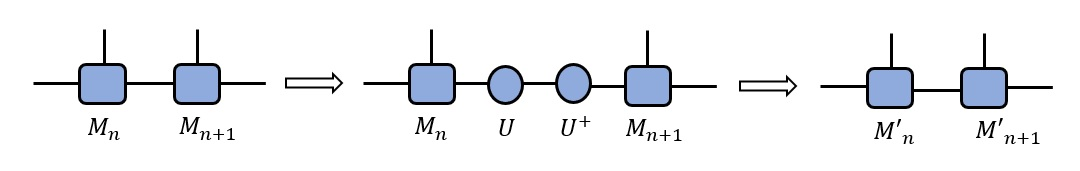
\includegraphics[scale=0.7]{5.矩阵乘积态规范自由度}
	   	\caption[9pt]{ 矩阵乘积态规范自由度}
	   	\label{fig:5}
	   \end{figure}
   
       首先定义张量的左右正交形式如图
       \begin{figure}[H]
       	\centering
       	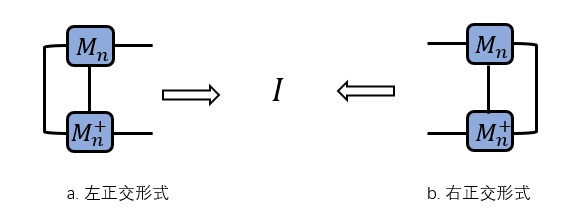
\includegraphics[scale=0.7]{6.MPS的左右正交形式}
       	\caption[9pt]{ 矩阵乘积态左右正交形式}
       	\label{fig:6}
       \end{figure}
        
       混合正交形式即选取一个格点或者格点间的连接(bond)为正交中心,正交中心左侧的张量都满足左正交形式,正交中心右侧的张量都满足右正交形式。例如选取正交中心为$l$格点和$l+1$格点间的连接,其构造如下\cite{vanderstraeten2019tangent}:
       对系数$C_{j_1,...,j_L}$从左端开始作SVD分解到l格点得到
       \begin{equation}C_{j_1,...,j_L}=\sum_{\alpha_l}(A^{j_1}...A^{j_l})_{\alpha_l}S_{\alpha_l,\alpha_l}(V^\dagger)_{\alpha_l,(j_{l+1},...,j_L)}.\end{equation}
       其中每个$A$矩阵是每次SVD分解中的U矩阵,满足左正交条件。将$V^\dagger$从右往左作SVD分解,将每一次得到的V矩阵作为$B^j_i$,最终得到
       \begin{equation}(V^\dagger)_{\alpha_l,(j_{l+1},...,j_L)}=\sum_{\alpha_1,...,\alpha_{L-1}}B_{\alpha_l,\alpha_{l+1}}^{j_{l+1}}...B_{\alpha_{L-1}}^{j_L}.\end{equation}
       所有的B矩阵都满足右正交条件,最终得到
       \begin{equation}C_{j_1,...,j_N}=A^{j_1}...A^{j_l}SB^{j_{l+1}}...B^{j_L}.\end{equation}
       \begin{figure}[H]
       	\centering
       	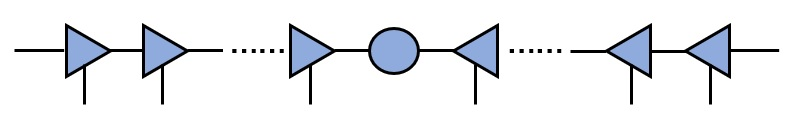
\includegraphics[scale=0.7]{7.矩阵乘积态混合正交形式}
       	\caption[9pt]{ 矩阵乘积态混合正交形式}
       	\label{fig:7}
       \end{figure}
       其中正交中心为$l$格点和$l+1$之间的奇异值,也可以用施密特分解的角度来理解:A子系统是从1到$l$格点,B子系统是$l+1$到$L$格点。如果我们引入向量
       \begin{equation}\begin{split} &|\alpha_l\rangle_A=\sum_{j_1,...,j_l}(A^{j_1}...A^{j_l})_{1,\alpha_l}|j_1,...,j_l\rangle
       \\ &|\alpha_l\rangle_B=\sum_{j_{l+1},...,j_L}(B^{j_{l+1}}...B^{j_L})_{\alpha_l,1}|j_{l+1},...,j_L\rangle .\end{split}\end{equation}
       
       因此波函数为\begin{equation}\Psi\rangle=\sum_{\alpha}S_\alpha|\alpha\rangle_A|\alpha\rangle_B.\end{equation}
	   
	\newpage
	{\centering\section{张量网络算法}}
	  \subsection{矩阵乘积算符}
	  密度矩阵重整化群算法(DMRG)依赖于将系统的哈密顿量表示成矩阵乘积算符(MPO)的形式。由MPS出发自然地得到MPO的形式,\cite{pirvu2010matrix}\cite{schollwock2011density}
	  \begin{equation}\hat{O}=\sum_{j_1,...,j_N;j'_1,...,j'_N} W^{[1]j_1j'_1}...W^{[N]j_Nj'_N}|j_1,...,j_N\rangle\langle j'_1,...,j'_N|.\end{equation}
	  其中$W^{[n]j_nj'_n}$是$D\times D$的矩阵,$|j_n\rangle,|j'_n\rangle$是$n$格点的基矢。
	  
	  MPO直接作用到MPS上得到的依然是MPS的形式
	  \begin{equation}\begin{split}
	  	\hat{O}|\Psi\rangle &=\sum_{j,j'}(W^{j_1,j'1}...W^{j_N,j'_N})(M^{j_1}...M^{j_N})|j_1,...,j_N\rangle \\
	  	&=\sum_{j,j'}\sum_{a,b}(W^{j_1,j'_1}_{1,b_1}...W^{j_N,j'_N}_{b_{N-1}b_N})(M^{j_1}_{1,a_1}...M^{j_N}_{a_{N-1},a_N})|j_1,...,j_N\rangle\\
	  	&=\sum_{j,j'}\sum_{a,b}(W_{1,b_1}^{j_1,j'_1}M^{j_1}_{1,a_1})...(W^{j_N,j'_N}_{b_{N-1}b_N}M^{j_N}_{a_{N-1},a_N})|j_1,...,j_N\rangle\\
	  	&=\sum_{j'}\sum_{a,b}N^{j'_1}_{(1,1),(b_1,a_1).}..N^{j'_N}_{b_{N-1},a_{N-1}}|j'_1,...,j'_N\rangle
	  	=\sum_{j'}N^{j'_1}...N^{j'_N}|j'_1,...,j'_N\rangle
	  .\end{split}\end{equation}
      图形示意为
      \begin{figure}[H]
      	\centering
      	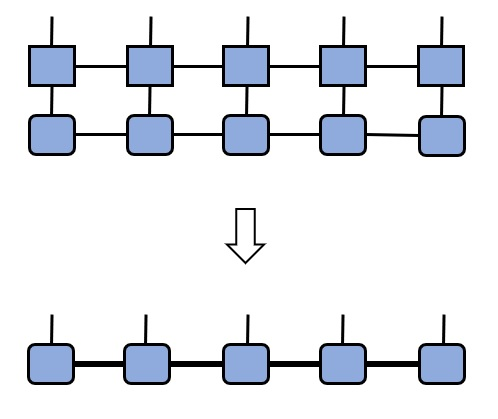
\includegraphics[scale=0.7]{8.MPO作用到MPS上}
      	\caption[9pt]{ MPO作用到MPS上}
      	\label{fig:8}
      \end{figure}
	  
	  \subsection{密度矩阵重整化群算法}
	  
	  密度矩阵重整化群(DMRG)算法由Steven White提出,随后不断演化形成了以MPS和MPO为范式的一套算法。DMRG是通过对MPS变分求出系统的基态,同时优化相邻格点的张量使得能量$\langle\Psi|H|\Psi\rangle$最小。在物理和化学的应用中,DMRG通常用来寻找多体系统哈密顿量的基态。它也可以扩展用来求解激发态,以及模拟非平衡的动力学演化。
	  
	  该算法核心是每个格点依次优化,优化方式为构造一个有效哈密顿量$H_{eff}$,求解出该哈密顿量的基态。使用SVD分解或其它矩阵正交分解使其回到MPS形式,在分解过程中可以对MPS做维度截断。接下来具体介绍该算法如何实现。\cite{schollwock2011density}
	  
	  {\heiti 第一步——构造有效哈密顿量}
	  
	  以第一个格点及相邻的第二个格点的优化为例,有效哈密顿量的构造方式为:将MPS中表示第一和第二个格点的张量去除,记为$|\Phi\rangle$.系统的哈密顿量用MPO表示。$H_{eff}=\langle\Phi| H|\Phi\rangle$
	  \begin{figure}[H]
	  	\centering
	  	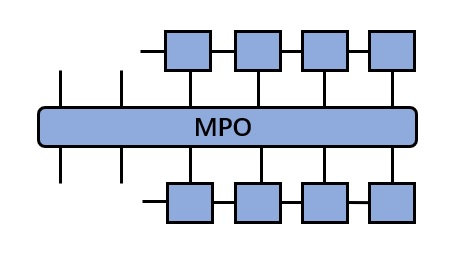
\includegraphics[scale=0.7]{9.有效哈密顿量示意}
	  	\caption[9pt]{ 有效哈密顿量示意}
	  	\label{fig:9}
	  \end{figure}
	  
	  {\heiti 第二步——求解有效哈密顿量基态}
	  上述的$H_{eff}$是一个六阶张量,通过重组使其变为二阶的矩阵。由于该矩阵维度很小,我们可以直接用Lanczos算法求解其基态。该基态为优化过后的第一个格点和第二个格点对应的张量。
	  
	  {\heiti 第三步——回归到MPS形式}
	  在获得第一个格点和第二个格点对应张量$B_{12}$后,我们需要将其回到MPS的形式,这样才能移动到下一个格点继续做优化。因此我们需要对$B_{12}$作SVD分解。
	  \begin{figure}[H]
	  	\centering
	  	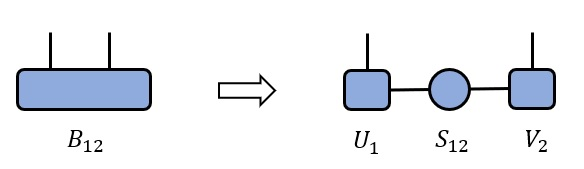
\includegraphics[scale=0.7]{10.SVD分解}
	  	\caption[9pt]{ SVD分解}
	  	\label{fig:10}
	  \end{figure}
  
      在SVD分解时作维度截断,保留$U_1$的前m列,$V_2$的前m行以及m个最大的奇异值。将截断后的$U_1$作为优化后的MPS第一个张量$M_1$,优化后的第二个张量$M_2=S_{12}V_2$。
      
      {\heiti 第四步——重复上述步骤依次优化其它格点}
      上面介绍了优化第一个和第二个格点的操作,接下来是对第二个和第三个格点进行优化。这样从左到右从1格点到N格点再从N个点优化回来到1格点称为一个sweep,重复多次sweep直到MPS收敛,我们便得到了系统的基态,这样同时优化两个格点的方法也称为two-site DMRG. 
	  
	  \subsection{时间演化块消减算法——TEBD}
	  在TEBD算法中,我们研究量子态的时间演化\cite{vidal2003efficient}:
	  \begin{equation}|\Psi(t)\rangle=U(t)|\Psi(0)\rangle.\end{equation}
	  时间演化算符$U$可以是实时演化算符$U(t)=exp(-itH)$,也可以是虚时演化算符$U(\tau)=exp(-\tau H)$。虚时演化可以用来计算系统的基态:
	  \begin{equation}|\Psi_{GS}\rangle=\lim_{\tau\to \infty}\frac{e^{\tau H}|\Psi_0\rangle}{||e^{\tau H}|\Psi_0\rangle||}.\end{equation}
	  TEBD算法利用了Suzuki-Trotter分解,它的一阶近似如下:
	  \begin{equation}e^{X+Y}\delta=e^{X\delta}e^{Y\delta}+O(\delta^2).\end{equation}
	  其中$X$和$Y$都是算符,$\delta$是一个小参数。我们可以将哈密顿量分解位两格点算符的求和$H=\sum_nh^{[n,n+1]}$,其中$h^{[n,n+1]}$是只作用到$n$和$n+1$格点上:
	  \begin{equation}H=\sum_{n odd}h^{[n,n+1]}+\sum_{n even}h^{[n,n+1]}.\end{equation}
	  
	  现在我们将时间分割成小份$\delta t\ll1$,考虑时间演化算符$U(\delta t)$,利用上述分解,可以将其展开成两格点算符的直积形式
	  \begin{equation}U(\delta t)\approx[\prod_{nodd}U^{[n,n+1]}(\delta t)][\prod_{neven}U^{[n.n+1]}(\delta t)].\end{equation}
	  其中$U^{[n,n+1]}(\delta t)=e^{-i\delta th^{[n,n+1]}}$。因此时间演化算符如下图所示,相继作用到MPS上。
	  \begin{figure}[H]
	  	\centering
	  	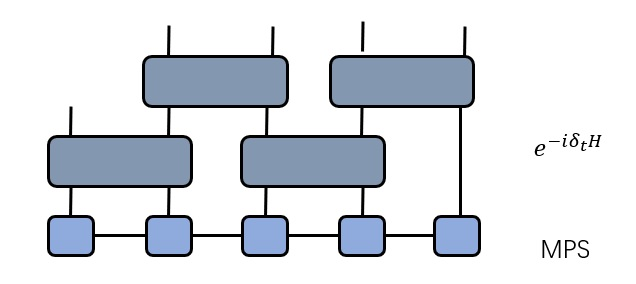
\includegraphics[scale=0.7]{15.Trotter分解}
	  	\caption[9pt]{将演化算符分解后与MPS作用示意}
	  	\label{fig:15}
	  \end{figure}
      
     接下来介绍TEBD算法\cite{hauschild2018efficient},同时更新相邻的两个格点。首先将波函数用混合正交形式表示,波函数系数$\Theta$为
     \begin{equation}\Theta_{\alpha_n\alpha_{n+2}}^{j_nj_{n+1}}=\sum_{\alpha_{n+1}}\Lambda_{\alpha_n\alpha_n}^{[n]}B_{\alpha_n\alpha_{n+1}}^{[n],j_n}B_{\alpha_{n+1}\alpha_{n+2}}^{[n+1],j_{n+1}}.\end{equation}
     将两点演化算符作用上去得到
     \begin{equation}\tilde{\Theta}_{\alpha_n\alpha_{n+2}}^{j_nj_{n+1}}=\sum_{j'_nj'_{n+1}}U_{j'_nj'_{n+1}}^{j_nj_{n+1}}\Theta_{\alpha_n\alpha_{n+2}}^{j'_nj'_{n+1}}.\end{equation}
     为了接下来的SVD分解,我们将$\Theta$重组为一个矩阵$\Theta_{j_n\alpha_n;j_{n+1}\alpha_{n+1}}$,如图所示:
     \begin{figure}[H]
     	\centering
     	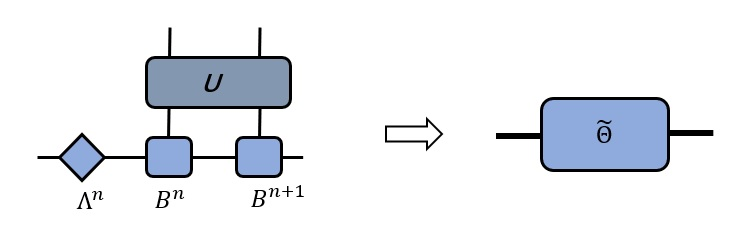
\includegraphics[scale=0.8]{16.TEBD1step}
     	\caption[9pt]{将时间演化算符作用到相应格点上,并合并指标重组为矩阵}
     	\label{fig:16}
     \end{figure}
     对矩阵$\tilde{\Theta}$作SVD分解,
     \begin{equation}\tilde{\Theta}_{j_n\alpha_n;j_{n+1}\alpha_{n+2}}=\sum_{\alpha_{n+1}}\tilde{A}_{j_n\alpha_n;\alpha_{n+1}}^{[n]}\tilde{\Lambda}_{\alpha_{n+1}\alpha_{n+1}}^{[n+1]}\tilde{B}_{\alpha_{n+1}j_{n+1}\alpha_{n+2}}^{[n+1]}.\end{equation}
     SVD后得到的张量满足混合正交形式,对角矩阵$\tilde{\Lambda}^{[n+1]}$包含了施密特分解值,可以用来计算纠缠熵。最后还回到最初的右正交形式:
     \begin{equation}\tilde{B}^{[n]}=(\Lambda^{[n]})^{-1}\tilde{A}^{[n]}\tilde{\Lambda}^{[n+1]},\qquad \tilde{B}^{[n+1]}=\tilde{B}^{[n+1]} .\end{equation}
     如图所示:
     \begin{figure}[H]
     	\centering
     	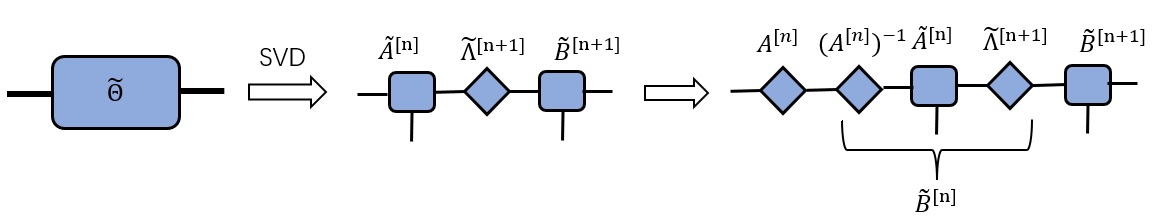
\includegraphics[scale=0.7]{17.TEBD2step}
     	\caption[9pt]{对$\tilde{\Theta}$作SVD分解,并还回最初的右正交形式}
     	\label{fig:17}
     \end{figure}
     
     完成一次上述更新后,新的MPS依然是正交形式。在演化过程中纠缠熵会随时间增加,因此连接维度应该指数增加。但我们选取了一个固定的维度$\chi_{max}$,因此随着时间演化,截断误差带来的影响会越来越大。如果我们采用TEBD的虚诗演化求解系统基态,算符$U$不是幺正的并且因此TEBD不能保证MPS的正交形式。但如果我们将时间步长取得非常小,施密特分解仍然能满足在长时情况下很好的近似。  
	
	
	  \subsection{含时变分原理}
	  MPS能够如此流行和成功的原因除了能够利用DMRG求解系统基态,它也能用来研究系统含时演化的动力学性质,例如时间演化块消减算法(TEBD)。TEBD算法中最重要的一点是对哈密顿量进行Lie-Trotter-Suzuki分解,$\hat{H}=\sum_i\hat{h_i}$。其中$\hat{h_i}$是局域格点的哈密顿量,可以有效地作用到MPS上。但TEBD有以下缺点:无法处理有长程相互作用的系统;无法避免Trotter分解带来的误差\cite{haegeman2011time}。
	  
	  因此另一个时间演化的方法是由Jutho Haegeman提出的基于MPS的含时变分原理(TDVP),核心思路是将薛定谔方程$\hat{H}|\Psi\rangle$投影到切空间。该方法可以处理长程相互作用。Jutho Haegeman在2011年最开始提出的算法需要对格拉姆矩阵求转置,该方法稳定性并不够好。于是在2016年他提出了一种优化算法,新算法基于对切空间投影算法进行Trotter分解,并且该算法和DMRG算法极其相似,可视为时间间隔为无穷大的one-site DMRG的虚时演化\cite{haegeman2011time}。
	  
	  先介绍含时变分原理,引入一个时间依赖的函数$A(t)$到薛定谔方程中得到
	  \begin{equation}\dot{A}^i|\partial_i\Psi(A(t))\rangle=-i\hat{H}|\Psi(A(t))\rangle.\end{equation}
	  其中方程左边是切向量$|\partial_i\Psi(A(t))\rangle$的线性组合,方程右边是希尔伯特空间中的某个向量,因此该方程无法得到$\dot{A}^i$的精确解。但可以通过最小化$||\dot{A}^i|\partial_i\Psi(A(t))\rangle+i\hat{H}|\Psi(A(t))\rangle||$得到最优近似。因此需要将$\hat{H}|\Psi\rangle$投影到切空间。
	  \begin{equation}\langle\partial_{\bar{j}}\Psi|\partial_i\Psi\rangle\dot{A}^i=-i\langle\partial_{\bar{j}}\Psi|\hat{H}|\Psi\rangle.\end{equation}
	  \begin{figure}[H]
	  	\centering
	  	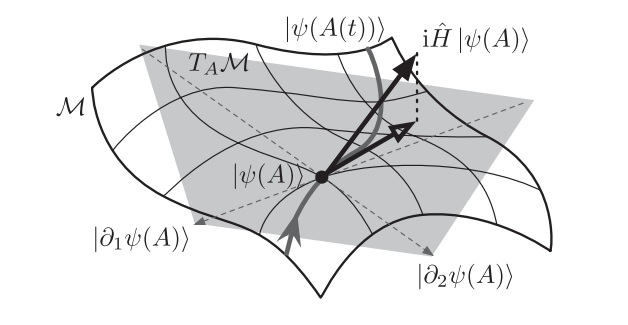
\includegraphics[scale=0.8]{11.TDVP示意}
	  	\caption[9pt]{ TDVP示意,图片源于参考文献}
	  	\label{fig:11}
	  \end{figure}
	  在介绍该算法如何实现之前,我们继续对混合正交形式的MPS进一步讨论。在之前叙述中,MPS的正交中心为仅包含奇异值的S矩阵,$|\Psi\rangle=\sum_{\alpha,\beta}[C(n)]_{\alpha,\beta}|\Phi_{L,\alpha}^{[1:n]}\rangle|\Phi_{R,\beta}^{[n+1:N]}\rangle$,它不包含格点的物理指标。同样我们可以把S矩阵和相邻的一个格点收缩,使得正交中心为包含格点物理指标的一个三阶张量,$|\Psi\rangle=\sum_{\alpha,j_n,\beta}[A_C^{s_n}(n)]_{\alpha,\beta}|\Phi_{L,\alpha}^{[1:n-1]}\rangle|j_n\rangle|\Phi_{R,\beta}^{[n+1:N]}\rangle$
	  \begin{figure}[H]
	  	\centering
	  	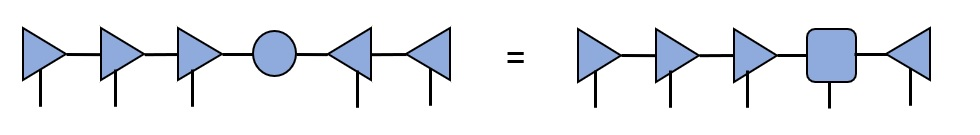
\includegraphics[scale=0.7]{12.MPS的两种混合正交形式}
	  	\caption[9pt]{ MPS的两种混合正交形式}
	  	\label{fig:12}
	  \end{figure}
      
      TDVP要求我们将薛定谔方程投影到MPS流形的切空间\cite{haegeman2016unifying},$\frac{d|\Psi(A)\rangle}{dt}=-i\hat{P}_T\hat{H}|\Psi(A)\rangle$。因此最重要的部分是将投影算符$\hat{P}_T$表示出来,文章推导得到
      \begin{equation}\hat{P}_T=\sum_{n=1}^{N}\hat{P}_L^{[1:n-1]}\otimes\hat{1}_n\otimes\hat{P}_R^{[n+1:N]}-\sum_{n=1}^{N-1}\hat{P}_L^{[1:n]}\otimes\hat{P}_R^{[n+1:N]}.\end{equation}
      其中
      \begin{equation}\begin{split}
      	\hat{P}_L^{[1:n]}&=\sum_{\alpha=1}^{D}|\Phi_{L,\alpha}^{[1:n]}\rangle\langle\Phi_{L,\alpha}^{[1:n]}|\\
      	\hat{P}_R^{[n:N]}&=\sum_{\beta=1}^{D}|\Phi_{R,\beta}^{[n:N]}\rangle\langle\Phi_{R,\beta}^{[n:N]}|.
      \end{split}\end{equation}
     
     \begin{figure}[H]
     	\centering
     	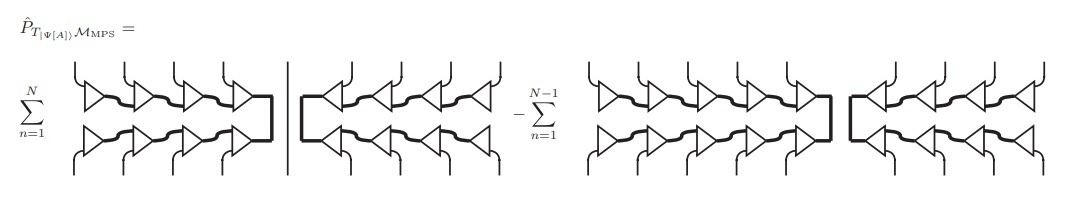
\includegraphics[scale=0.75]{13.投影算符表示}
     	\caption[9pt]{ 投影算符表示,图片源于参考文献}
     	\label{fig:13}
     \end{figure}
     
     于是我们可以将$\hat{P}_T\hat{H}|\Psi(A)\rangle$表示出来,利用MPS的两种混合正交表示形式以及one-site和zero-site有效哈密顿量。
     \begin{figure}[H]
     	\centering
     	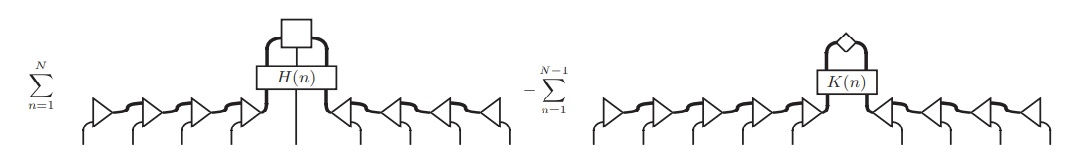
\includegraphics[scale=0.75]{14.TDVP方程等号右端}
     	\caption[9pt]{ TDVP方程等号右端,图片源于参考文献}
     	\label{fig:14}
     \end{figure}
     将$|\Psi\rangle$分别用两种混合正交形式表示,可以得到对应的微分方程。例如对于投影算符$\hat{P}_L^{[1:n-1]}\otimes\hat{1}_n\otimes\hat{P}_R^{[n+1:N]}$,并将$|\Psi\rangle$用含格点n的正交形式表示,可以得到$A_C(n,t)$的演化方程
     \begin{equation}A_C(n,t)=exp[-iH(n)t]A_C(n,0).\end{equation}
     同样,对于投影算符$\hat{P}_L^{[1:n]}\otimes\hat{P}_R^{[n+1:N]}$,并将$|\Psi\rangle$用不含格点n的正交形式表示,得到$C(n,t)$的演化方程
     \begin{equation}C(n,t)=exp[=iK(n)t]C(n,0).\end{equation}
     
     具体算法为:从n=1格点开始将$A_C(n)$按上述方程演化$\delta t$时间。演化后进行正交分解,$A_C^s(n)=A_L^s(n)C(n)$。将$C(n)$按照上述方程时间反演,将演化后的$C(n)$吸收到下一个格点,$A_C^s(n+1)=C(n)A_R^s(n+1)$。该算法和one-site DMRG算法非常相似,主要有两点不同:一是将DMRG中求有效哈密顿量基态变为时间演化形式;二是多了一个$C(n)$的时间反演,以及将其吸收到下一个格点。
	  	
	\newpage
    {\centering\section{量子淬火(Quantum quench)动力学研究}     }

    对于孤立系统非平衡动力学研究发现对于现有的理论和实验提出了挑战,提出了许多基本的问题以及各种应用。所谓量子淬火研究(quantum quench)指的是系统从一个初态开始演变,该初态需要满足是一个平移不变哈密顿量的基态。然而控制该系统演化的哈密顿量与基态对应的哈密顿量并不相同。
    
    在多体系统的研究中,quench是一个重要并且具有挑战性的问题:(i)跨相变quench的研究,例如系统的初态具有某种长程关联,如果quench之后的哈密顿量没有这种关联,那么关联函数应该如何演变呢。(ii)非平衡系统热化研究,将一个系统在quench之后进行长时演化,它的子系统的热化形式是如何的,会达到平衡态还是非平衡态。
    
      \subsection{一维横场伊辛模型}
      一维横场伊辛的哈密顿量为
      \begin{equation}\hat{H}=-J\sum_j \hat{\sigma}_j^z \hat{\sigma}_{j+1}^z- h\sum_j\hat{\sigma}_j^x.\end{equation}
      
      \noindent{\heiti$h=0$极限}
      
      当横场$h=0$,耦合系数$j>0$时,体系只剩下伊辛耦合部分,体系的基态为全部自旋向上或者全部自旋向下的铁磁态,$|\Psi_0\rangle=\prod_j|\uparrow\rangle$或者$|\Psi_0\rangle=\prod_j|\downarrow\rangle$。
      
      \noindent{\heiti$J=0$极限}
      
      体系只有一个横场项,系统的基态为自旋全部朝向X的态,$|\Psi_0\rangle=\prod_j|\to\rangle_j=\prod_j\frac{1}{\sqrt{2}}(|\uparrow\rangle_j+|\downarrow\rangle_j)$
      
      通过以上两种极端情况讨论可以发现,当$J/h\gg1$的区域,系统处于(z方向)铁磁态,对称性破缺。而在$J/h\ll1$的区域,体系处于无序态,也就是z方向的磁化为零$\langle\sigma^z\rangle$这样当我们调节$J/h$,体系存在从铁磁态到顺磁态的相变。显然在零温时体系不存在热涨落,这里的相变完全是由量子力学效应驱动的,将其称为量子相变。
      
      \subsubsection{基态能量及磁化}
      一维的量子自旋模型可以通过Jordan-Wigner变换改写为费米子模型,在这里的横场伊辛模型最后对应于自由费米子问题,体系是可以精确求解的\cite{sachdev2011quantum}。为了便于求解,我们把体系的坐标轴绕y轴旋转90度即$x\to-z,z\to x,y\to y$,这样体系的哈密顿量变为
      \begin{equation}\hat{H}=-J\sum_j\hat{\sigma}_j^x \hat{\sigma}_{j}^x + h\sum_j\sigma_{j}^z .\end{equation}
      Jordan-Wigner变换的定义为
      \begin{equation}\sigma_j^+=\prod_{l<j}(1-2\psi_l^+\psi_l)\psi_j, \qquad \sigma_j^-=\prod_{l<j}(1-2\psi_l^+\psi_l)\psi_j^+ .\end{equation}
      利用该变换得到哈密顿量的形式
      \begin{equation}\begin{split} \hat{H}&=-J\sum_j( \hat{f}^+_j\hat{f}^+_{j+1} + \hat{f}^+_j\hat{f}_{j+1} + \hat{f}^+_{j+1}\hat{f}_j + \hat{f}_{j+1}\hat{f}_j ) + 2h\sum_j(\hat{f}^+_j\hat{f}_j) \\ &= -J\sum_j( \hat{f}^+_j\hat{f}^+_{j+1} + \hat{f}^+_j\hat{f}_{j+1} + H.c.)+ 2h\sum_j(\hat{f}^+_j\hat{f}_j).\end{split} \end{equation}
      
      当考虑周期边界条件,系统满足平移不变性,因此可以利用傅里叶变换来对角哈密顿量。费米子算符的傅里叶变换为:
      \begin{equation}\hat{f}_j=\frac{1}{\sqrt{N_s}}\sum_ke^{ikR_j}\hat{f}_k.\end{equation}
      其中$N_s$是系统的格点总数,$R_j$是第j个格点的位置,动量$k$在第一布里渊区取值$k\in[-\pi/a,\pi/a]$,a是晶格常数。这样哈密顿量可以写为:
      \begin{equation}\hat{H}=\sum_k [(-2J\cos (ka)+2h)\hat{f}_k^+\hat{f}_k-Je^{ika}\hat{f}_k^+\hat{f}^+_{-k} -Je^{-ika}\hat{f}_{-k}\hat{f}_{k}-hN_s ].\end{equation}
      我们将常数项省略,定义$\varepsilon_k= -2J\cos k+2h,\Delta_k=2J\sin k$,并且把$k<0$的求和替换为$-k$得到
      \begin{equation} \hat{H}=\sum_{k>0}[\varepsilon_k(\hat{f}_k^+\hat{f}_k + \hat{f}_{-k}^+\hat{f}_{-k})-i\Delta_k\hat{f}_k^+\hat{f}_{-k}^+ + i\Delta_k\hat{f}_{-k}\hat{f}_k] .\end{equation}
      进一步写成矩阵形式
      \begin{equation}\hat{H}= \begin{pmatrix} \hat{f}_k^+&\hat{f}_{-k} \end{pmatrix} \begin{pmatrix} \varepsilon_k&-i\Delta_k\\i\Delta_k&-\varepsilon_k  \end{pmatrix} \begin{pmatrix} \hat{f}_k\\\hat{f}_{-k}^+ \end{pmatrix}+\sum_{k>0}\varepsilon_k .\end{equation}
      
      我们进一步引入Bogoliubov变换将哈密顿量对角化。引入费米子算符$\alpha_k$和$\beta_k^+$:
      \begin{equation}\begin{pmatrix} \hat{\alpha}_k\\ \hat{\alpha}_{-k}^+\end{pmatrix}= \begin{pmatrix} \cos\theta_k&-i\sin\theta_k\\-i\sin\theta_k&\cos\theta_k\end{pmatrix} \begin{pmatrix} \hat{f}_k\\\hat{f}_{-k}^+ \end{pmatrix} = \hat{U}\begin{pmatrix} \hat{f}_k\\\hat{f}_{-k}^+ \end{pmatrix}.\end{equation}
      将其带入哈密顿量
      \begin{equation}\hat{H}=\sum_{k>0}\begin{pmatrix} \hat{\alpha}_k^+&\hat{\alpha}_{-k}\end{pmatrix} \hat{U}\hat{h}_k\hat{U}^{-1}\begin{pmatrix} \hat{\alpha}_k^+\\\hat{\alpha}_{-k}\end{pmatrix},\quad \hat{h}_k=\begin{pmatrix} \varepsilon_k&-i\Delta_k\\i\Delta_k&-\varepsilon_k\end{pmatrix} .\end{equation}
      我们要求对角化哈密顿量,即要求$\hat{U}\hat{h}_k\hat{U}^{-1}$非对角项为0.
      \begin{equation}\hat{U}\hat{h}_k\hat{U}^{-1}=\begin{pmatrix} \varepsilon_k\cos2\theta_k+\Delta_k\sin2\theta_k&\varepsilon_k\sin2\theta_k-\Delta_k\cos2\theta_k\\-\varepsilon_k\sin2\theta_k+\Delta_k\cos2\theta_k&-\varepsilon_k\cos2\theta_k-\Delta_k\sin2\theta_k \end{pmatrix} .\end{equation}
      因此要求
      \begin{equation}\varepsilon_k\sin2\theta_k-\Delta_k\cos2\theta_k=0\Rightarrow\frac{\Delta_k}{\varepsilon_k}=\frac{\sin2\theta_k}{\cos2\theta_k} .\end{equation}
      此时体系的哈密顿量为
      \begin{equation}\hat{H}=\sum_{k}\sqrt{\varepsilon_k^2+\Delta_k^2}(\hat\alpha_k^+\hat{\alpha_k})+\sum_{k>0}(\varepsilon_k-\Delta_k) .\end{equation}
      
      \noindent{\heiti 基态能量}
      
      系统的色散关系为 $E_k=\sqrt{\varepsilon_k^2+\Delta_k^2}=2J\sqrt{1+(h/J)^2-2(h/J)\cos k}$,当$h/J$=1时,系统存在无能隙激发,这种无能隙激发将会导致自由能及其他物理量的热力学奇异性,说明$h/J=1$是体系的临界点。$T=0$时体系的基态是
      \begin{equation}E_g=\frac{1}{N_s}\sum_{k>0}(\varepsilon_k-\sqrt{\varepsilon_k^2+\Delta_k^2})=\int_{0}^{\pi}(\varepsilon_k-\sqrt{\varepsilon_k^2+\Delta_k^2})\frac{dk}{2\pi}.\end{equation}
      
      利用DMRG算法求解一维横场伊辛模型的基态能量并与解析的结果相比较,如图18(a)
      \begin{figure}[H]
      	\centering
      	\begin{minipage}{0.49\linewidth}
      		\centering
      		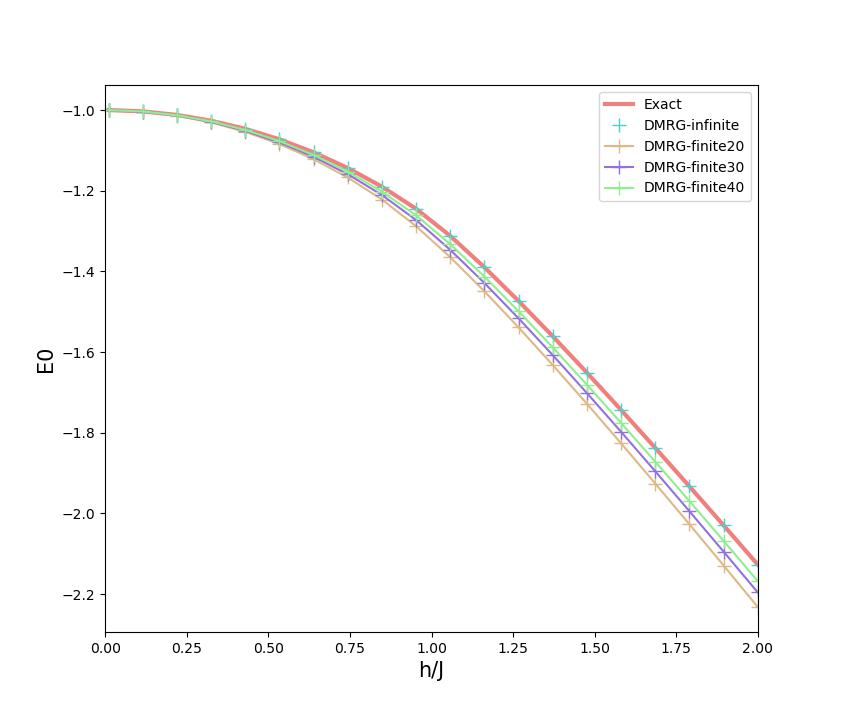
\includegraphics[width=260pt]{TFIM基态}
      		\title{(a)}
      		\label{fig:18}
      	\end{minipage}%
      	\begin{minipage}{0.49\linewidth}
      		\centering
      		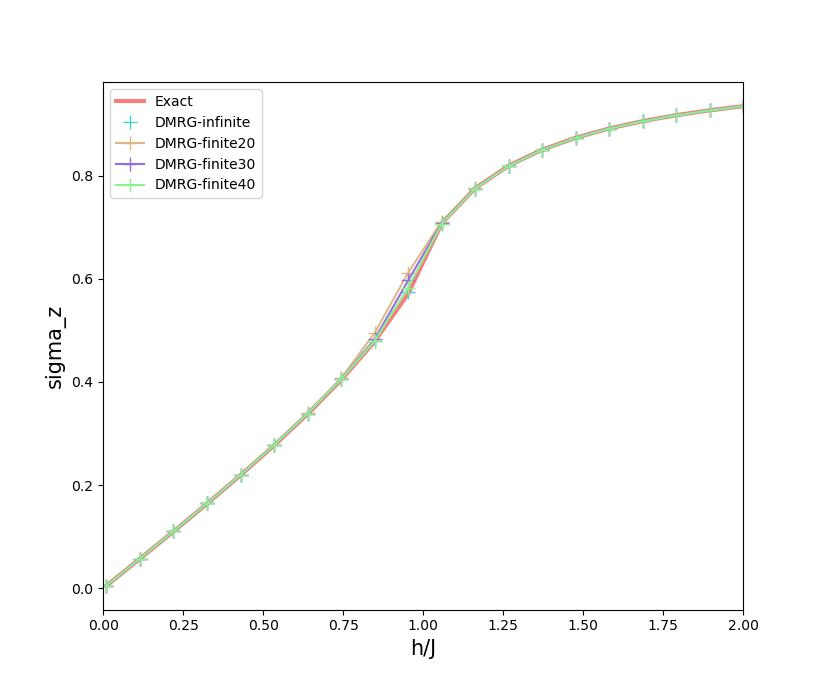
\includegraphics[width=260pt]{TFIMSz0}
      		\title{(b)}
      		\label{fig:19}
      	\end{minipage}
      \caption[9pt]{横轴为$h/J$,(a)图纵轴为基态能量$E_0$,(b)图纵轴为基态磁化$\langle\sigma_z\rangle$,图中曲线分别有解析精确值,以及格点数为20,30,40和无限长的DMRG算法}
      \end{figure}
      
      在算法中我们采取的是开放边界条件,其中infinite-DMRG可以理解为两个格点的系统采取周期性边界条件。可以看出,随着格点数量的增加,基态能量和解析结果拟合得越好,边界效应所带来的影响越小。
      
      \noindent{\heiti $\langle\sigma_z\rangle$磁化}
      
       $\langle\sigma_z\rangle=\frac{1}{N}\sum_j\sigma_{j}$用费米子算符$\alpha_k$和$\alpha_{-k}$表示出来:
       \begin{equation} \begin{split} \sigma_z&=1-\frac{2}{N}\sum_kf_k^+f_k\\ &=1-\frac{2}{N}\sum_k \cos^2\theta_k\alpha_k^+\alpha_k- \sin^2\theta_k\alpha_{-k}^+\alpha_{-k}+\sin^2\theta_k+\cos\theta_k\sin\theta_k(\alpha_k^+\alpha_{-k}^++\alpha_{-k}\alpha_k). \end{split} \end{equation}
       利用上式,可以得到基态z方向磁化$\langle GS|\sigma_z|GS\rangle=1-\frac{2}{N}\sum_k \sin^2\theta_k=\frac{2}{N}\sum_q\cos2\theta_k$
       
       由图18(b)可以看出,无论是有限格点还是无限格点的DMRG算法都能很好地拟合$\langle\sigma_z\rangle$
       
      \noindent{\heiti 寻找相变点}
      
      系统的激发能量为:
      \begin{equation}
      	E_k=\sqrt{\varepsilon_k^2+\Delta_k^2}=2J\sqrt{1+g^2-2g\cos k}.
      \end{equation}
      体系仅在$g=h/J=1$时存在无能隙激发,说明该点是体系的临界点,而在其他情况下激发能都是有限值,这种无能隙激发将会导致物理量的热力学奇异性。我们可以通过数值算法得到不同g值下的热力学量来验证一维横场伊辛的相变点\cite{hauschild2018efficient}。
      
       \begin{figure}[H]
      	\centering
      	\begin{minipage}{0.49\linewidth}
      		\centering
      		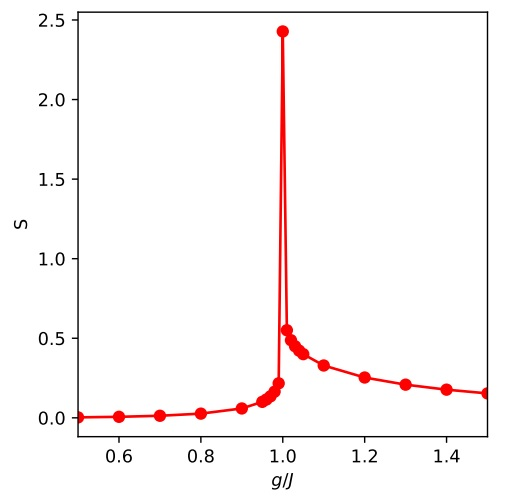
\includegraphics[width=1\linewidth, height=230pt]{tfi_tran1}
      		\title{(a)纠缠熵S随$h/J$变化}
      		\label{fig:29}
      	\end{minipage}
      	\begin{minipage}{0.49\linewidth}
      		\centering
      		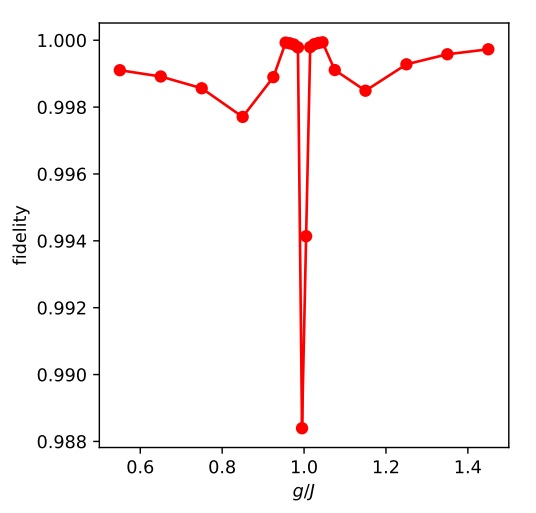
\includegraphics[width=1\linewidth, height=230pt]{tfi_tran2}
      		\title{(b)保真度$\langle\Psi|\Psi\rangle$随$h/J$变化}
      		\label{fig:30}
      	\end{minipage}
      
           	
      \begin{minipage}{0.49\linewidth}
      	\centering
      	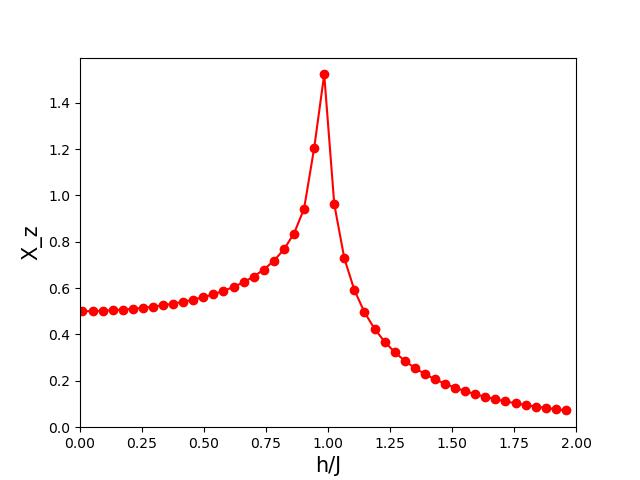
\includegraphics[width=1\linewidth, height=240pt]{tfi_tran4}
      	\title{(c)磁化率$\chi_z$随$h/J$变化}
      	\label{fig:31}
      \end{minipage}
       
      	\caption[9pt]{相变点呈现出奇异性}
      \end{figure}
  
  由图19可以看出在相变点附近,基态的纠缠熵和外场方向磁化率为极大值,保真度为极小值。可以明显地看出在相变点附近的基态与其他情况下基态的明显不同。另外在临界点附近,各类物理量显示出显著的幂律行为,相应的幂指数称为临界指数。不同物理系统的临界指数可能完全相同,称为普适类,即虽然物理系统的微观结构和宏观物理不尽相同,但当它们接近临界点时,它们的相变行为是类似的,具有相同的临界指数。因此我们可以验证当$J=1$时,在临界点$h=h_c=1$时的临界指数。在一维横场伊辛中,横向磁化$\langle\sigma_x\rangle$满足:$\langle\sigma_x\rangle\sim(h-h_c)^\beta, \quad \beta=1/8$。
  
  
   \begin{figure}[H]
   	\centering
   	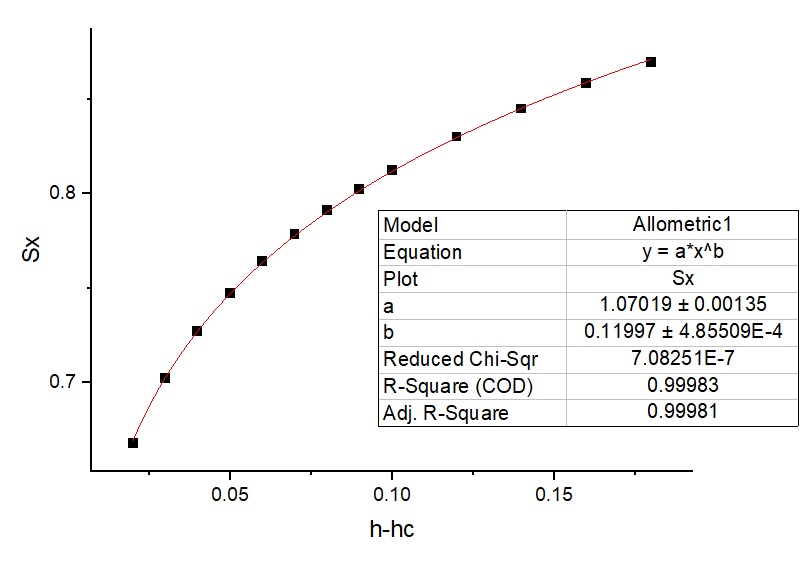
\includegraphics[scale=0.7]{tfi_tran3}
   	\caption[9pt]{$\langle\sigma_x\rangle\sim(h-h_c)^\beta$,拟合得到$\beta$}
   \end{figure}
   通过拟合得到临界指数$\beta$=0.11997,与精确值1/8接近。
   
   
      

       \subsubsection{淬火后时间演化}
      \noindent{\heiti 解析求解波函数时间演化形式}
      
      我们可以解析得到一维横场伊辛模型z方向磁化$\langle\sigma_z\rangle$在淬火后时间演化形式。首先我们需要得到淬火之前的基态波函数
      \begin{equation}\alpha_k|GS\rangle =0 \quad \Rightarrow \quad |GS\rangle=\prod_{k>0}[\cos\theta_k+\sin\theta_k\hat{f}_k^+\hat{f}_{-k}^+]|0\rangle .\end{equation}
      
      量子淬火意味着伊辛模型的纵场项强度突然发生变化,即$h\to h'$。经过同样的Jordan-Wigner变换以及Bogoliubov变换,可以得到$H(h)\to H(h')=\sum_{k}\tilde{E_k}(\tilde{\alpha}_k^+\tilde{\alpha}_{-k}-\frac{1}{2})+const$,因此可以得到quench前后费米子算符的关系
      \begin{equation} \begin{pmatrix} f_q\\f^+_{-q} \end{pmatrix}=\begin{pmatrix} \cos\theta_k & \sin\theta_k\\ -\sin\theta_k& \cos\theta_k \end{pmatrix}
      \begin{pmatrix} \alpha_k\\\alpha_{-k}^+ \end{pmatrix} = \begin{pmatrix} \cos\tilde\theta_k & \sin\tilde\theta_k\\ -\sin\tilde\theta_k& \cos\tilde\theta_k \end{pmatrix} \begin{pmatrix} \tilde\alpha_k\\\tilde\alpha_{-k}^+ \end{pmatrix} .\end{equation}
      
      \begin{equation}\Rightarrow\quad \begin{pmatrix} \alpha_k\\ \alpha_{-k}^+ \end{pmatrix}=\begin{pmatrix} \cos\beta_k&-\sin \beta_k\\ \sin\beta_k&\cos\beta_k \end{pmatrix} \begin{pmatrix} \tilde\alpha_k\\ \tilde\alpha_{-k}^+  \end{pmatrix}  .\end{equation}
      其中$\beta_k=\theta_k-\tilde{\theta}_k$,因此quench前的基态表示为
      \begin{equation}|GS\rangle_h= \prod_{k>0}(\cos\beta_k+\sin\beta_k\tilde{\alpha}_k^+\tilde{\alpha}_{-k}^+)|\tilde{0}\rangle .\end{equation}
      其中$\tilde{\alpha}|\tilde{0}\rangle=0$,  因此quench$(h\to h')$后,波函数的含时演化为
      \begin{equation}\begin{split}|\Psi_{h\to h'}(t)\rangle &=e^{-i\int H(h')dt}|GS\rangle_h \\ &=\prod_{k>0}(\cos\beta_k+\sin\beta_ke^{-i2\tilde{E}_qt}\tilde{\alpha}_k^+\tilde{\alpha}_{-k}^+)|\tilde 0\rangle \end{split}.\end{equation}
      
      \noindent{\heiti $\langle\sigma_z\rangle$在quench$(h\to h')$后时间演化}
      
      \begin{equation} \begin{split} \langle\Psi(t)|\sigma_z|\Psi(t)\rangle&=1-\frac{2}{N}\sum_k\langle\Psi(t)|\alpha_k^+\alpha_k|\Psi(t)\rangle\\ &=
      \frac{1}{N}\sum_k\cos\tilde{\theta_k}-\frac{4}{N}\sum_{k>0}\langle\Psi(t)|\cos^2\tilde{\theta}_k\tilde{\alpha}_k^+\tilde{\alpha}_k-\sin^2\tilde\theta_k\tilde\alpha_{-k}^+\tilde\alpha_{-k}\\&+\cos\tilde\theta_k\sin\theta_k(\tilde\alpha_k^+\tilde\alpha_{-k}+\tilde\alpha_{-k}\tilde\alpha_k)|\Psi(t)\rangle. \end{split} \end{equation}
      最终求解得到
      \begin{equation}\langle\Psi(t)|\sigma_z|\Psi(t)\rangle=\frac{2}{N}\sum_{k>0}[\cos2\beta_k\cos\tilde\theta_k-\sin2\beta_k\sin\tilde\theta_k\cos(2t\tilde E_q)] .\end{equation}
      
      利用DMRG-infinite算法求解系统系统基态,再改变哈密顿量的横场项,实现量子淬火(quntum quench),利用TEBD-infinite研究淬火后$\langle\sigma_z\rangle$的含时演化。如图
      
     \begin{figure}[H]
     	\centering
     	\begin{minipage}{0.49\linewidth}
     		\centering
     		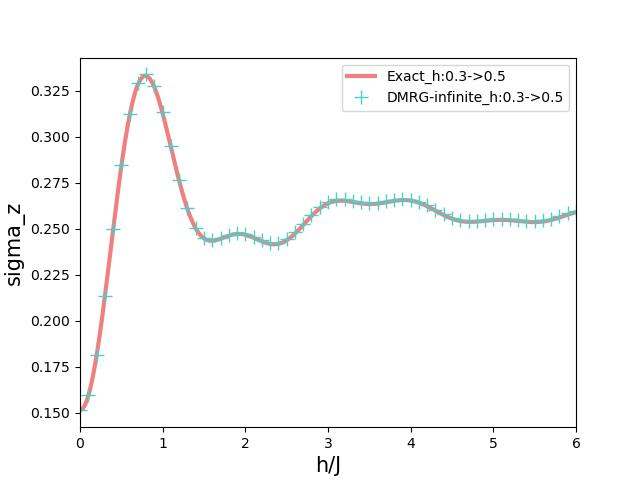
\includegraphics[width=0.9\linewidth]{TFIMSzt1}
     		\title{(a)$J=1,h:0.3\to0.5$}
     		\label{fig:20}
     	\end{minipage}
     	\begin{minipage}{0.49\linewidth}
     		\centering
     		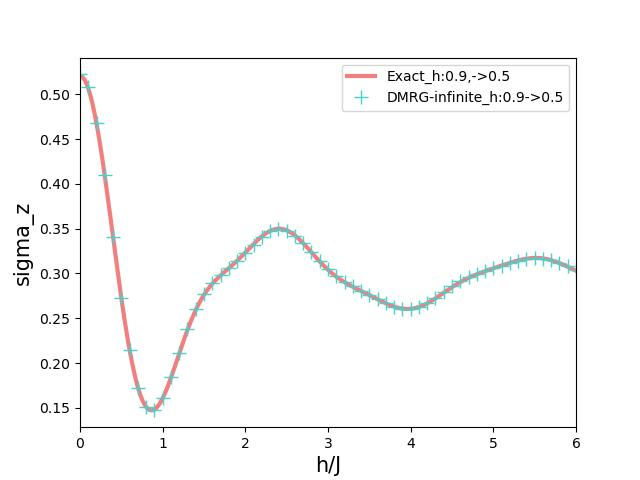
\includegraphics[width=0.9\linewidth]{TFIMSzt2}
     		\title{(b)$J=1,h:0.9\to0.5$}
     		\label{fig:21}
     	\end{minipage}
     	
     	\begin{minipage}{0.49\linewidth}
     		\centering
     		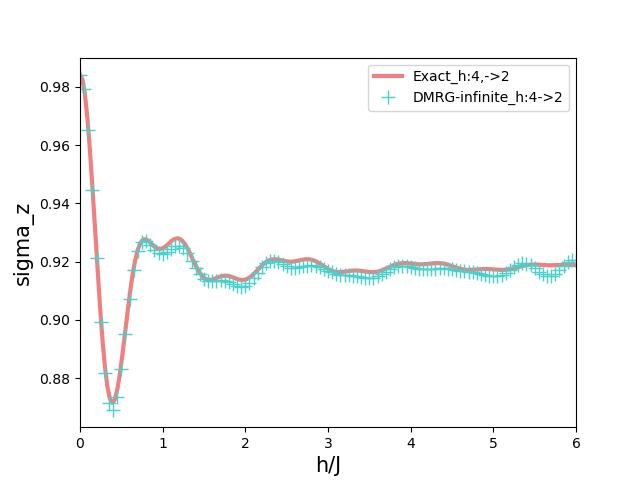
\includegraphics[width=0.9\linewidth]{TFIMSzt3}
     		\title{(c)$J=1,h:4\to2$}
     		\label{fig:22}
     	\end{minipage}
     	\begin{minipage}{0.49\linewidth}
     		\centering
     		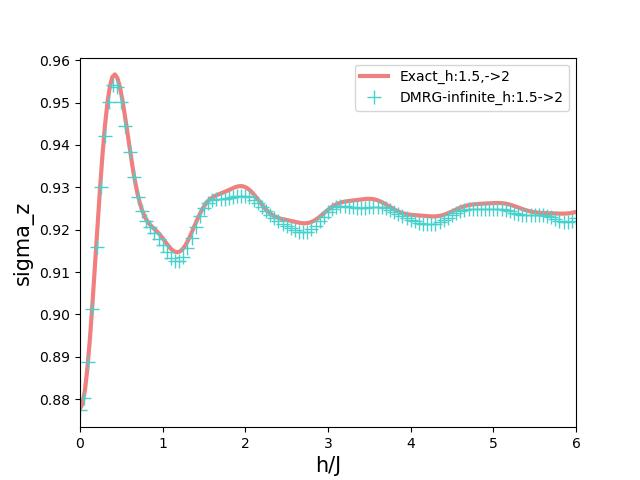
\includegraphics[width=0.9\linewidth]{TFIMSzt4}
     		\title{(d)$J=1,h:1.5\to2$}
     		\label{fig:23}
     	\end{minipage}
       \caption[9pt]{求解不同quench状态下的演化}
     \end{figure}
    从图中可以看出我们的DMRG+TEBD(infinite)算法能够很好的模拟quench动力学行为,但是由于TEBD算法存在误差,包括Trotter分解中只采用了一阶近似以及固定维度截断带来的误差,该含时演化在T较大时与解析结果偏差较大。从下图20(a)中可以看见当$t>5$左右时,误差已经比较明显,出现了振荡的情形。图20(b)采取了和图20(a)一样的quech模型$(h:1.5\to2)$,但相较于(a)中30的截断维度,(b)采取的截断维度为200。可以保留更多的SVD分解时的奇异值,即保留了更多的纠缠信息,因此时间演化更精准。
         
     \begin{figure}[H]
     	\centering
     	\begin{minipage}{0.49\linewidth}
     		\centering
     		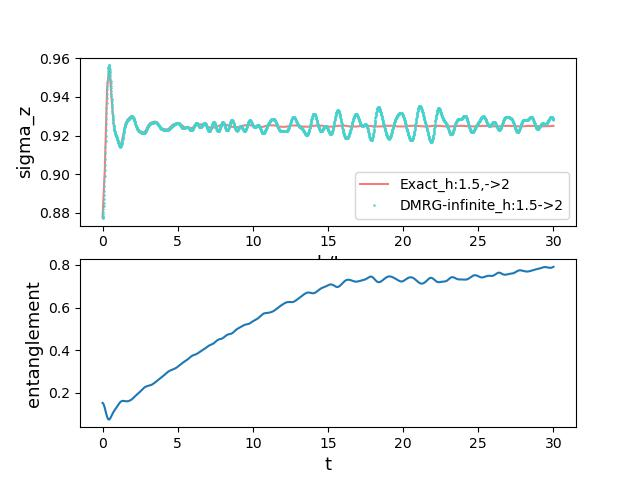
\includegraphics[width=1\linewidth, height=230pt]{ee1}
     		\title{(a)$h:1.5\to2$,固定截断为30}
     		\label{fig:29}
     	\end{minipage}
     	\begin{minipage}{0.49\linewidth}
     		\centering
     		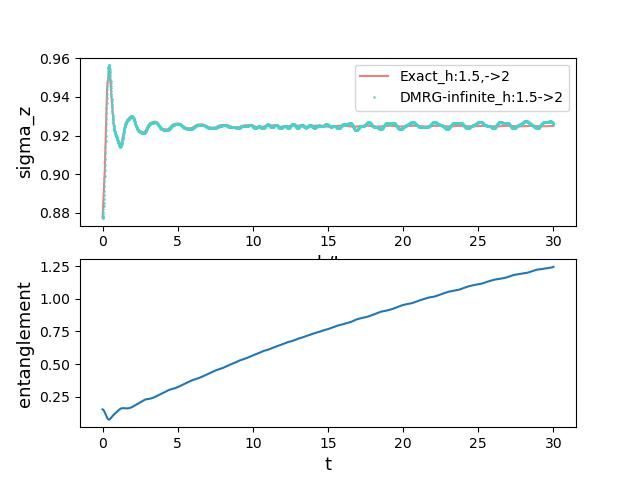
\includegraphics[width=1\linewidth, height=230pt]{ee2}
     		\title{(b)$h:1.5\to2$,固定截断为100}
     		\label{fig:30}
     	\end{minipage}
     	
     	\begin{minipage}{0.49\linewidth}
     		\centering
     		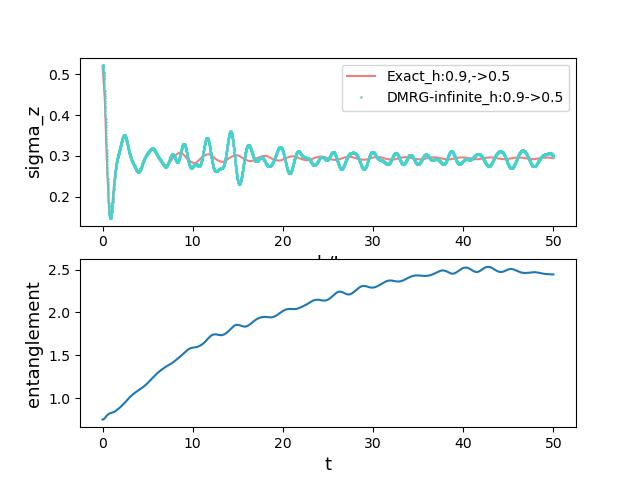
\includegraphics[width=1\linewidth, height=230pt]{ee4}
     		\title{(c)$h:0.9\to0.5$,固定截断为30}
     		\label{fig:31}
     	\end{minipage}
     	\begin{minipage}{0.49\linewidth}
     		\centering
     		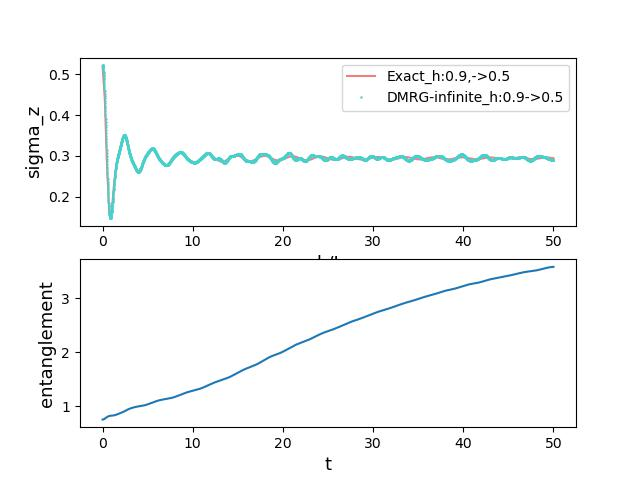
\includegraphics[width=1\linewidth, height=230pt]{ee3}
     		\title{(d)$h:0.9\to0.5$,固定截断为100}
     		\label{fig:32}
     	\end{minipage}
     	\caption[9pt]{求解不同quench状态下纠缠熵的演化}
     \end{figure}
 
 由于更大的截断维度意味着可以在SVD分解时保留更多的奇异值,也能得到更大的饱和纠缠熵。因此我们接下来研究纠缠熵在quench后随时间演化形式,下图得到了两种quench状态下,两种不同截断维度得到的$\sigma_z$随时间演化以及对于的纠缠熵随时间增加形式。可以看出,更大的截断维度下,纠缠熵的增加更快,并且能够达到的饱和纠缠熵更大。
     

     同样我们可以采用DMRG+TDVP算法\cite{fishman2020itensor}做quech动力学演化数值模拟,如图26所示,其中蓝色实线是解析值,红色$+$为DMRG+TDVP算法的数值解。其中DMRG和TDVP算法选取的总格点数为30,固定截断维度为30.可以看到由于固定截断维度取值较小,在$t>4$左右出现误差。
     \begin{figure}[H]
     	\centering
     	\begin{minipage}{0.49\linewidth}
     		\centering
     		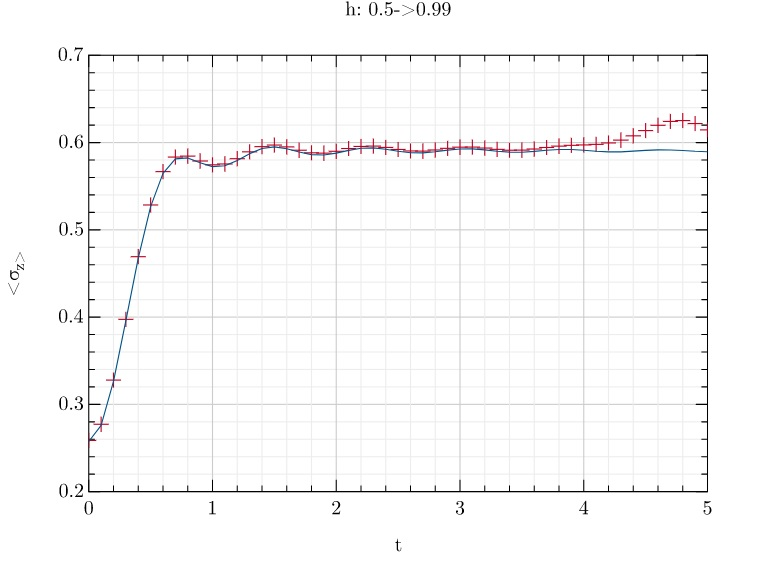
\includegraphics[width=1\linewidth, height=170pt]{TFIMSzt7}
     		\title{(a)}
     		\label{fig:33}
     	\end{minipage}
     	\begin{minipage}{0.49\linewidth}
     		\centering
     		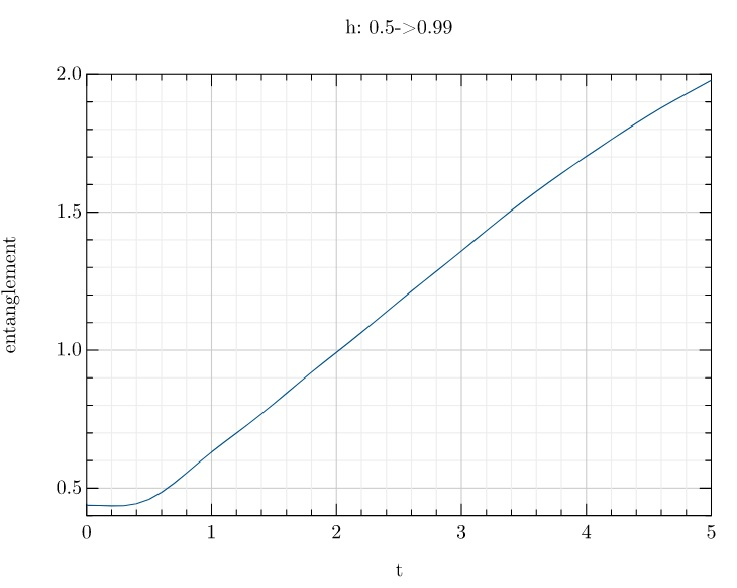
\includegraphics[width=1\linewidth, height=170pt]{tdvpe}
     		\title{(b)}
     		\label{fig:34}
     	\end{minipage}
        \caption{DMRG+TDVP,(a)图为$\sigma_z$随时间演化,其中蓝线为解析值,红线为数值解;(b)图为纠缠熵随时间增加}
     \end{figure}

      
      \subsection{一维XXZ自旋关联函数}
      我们考虑一维自旋$\frac{1}{2}$的XXZ链,有如下哈密顿量
      \begin{equation}  H(\Delta)=\sum_{j=1}^{L}(S_j^xS_{j+1}^x+S_j^yS_{j+1}^y+\Delta S_j^zS_{j+1}^z) .\end{equation}
      该系统在热力学极限下的性质为:当$|\Delta|<1$,系统是量子临界;当$\Delta>1$,系统基态为反铁磁态;当$\Delta<-1$,系统基态为铁磁态,激发有能隙\cite{collura2015quantum}。
      
      在接下来的讨论中,我们将系统系统处于XX模型$(\Delta_0=0)$的基态$|\Psi_0\rangle$,在t=0时,给系统施加一个z方向外场$\Delta\in(-1,1)$。接下来我们可以用数值方法来研究模型的自旋关联函数并与Luttinger Liquid理论得到的解析表达式相比较。
      
      在统计力学中,关联函数可以衡量系统的有序程度。关联函数刻画了不同时间不同空间的微观变量,比如自旋和密度,是如何联系起来的。具体来说,关联函数能够量化描述一个微观变量是如何随另一个空间和时间熵的变量而变化。
      
      首先同样用DMRG模型求解得到XX模型的基态,其中选取的总格点数为50,固定维度为30.计算出其基态能量为$E_0=-0.314727$与解析值$E_{XX}=1/\pi$相差$1.1\%$。如果采用iDMRG求解得到基态能量$E'_0=0.31830074$,误差为$0.003\%$. 
      
      利用该MPS作为基态,我们可以进行实时演化,选取时间步长$dt=0.1$,固定截断维度为30. 由于纠缠熵随时间演化迅速增加,我们需要不断增加截断维度来精确的描述系统演化。但由于计算机性能限制,我们选取了较小的截断维度,用来模拟短时间的含时演化。
      
      \noindent{\heiti 横向自旋关联函数 $\langle S_i^xS_j^x\rangle$ }
      
      利用Luttinger Liquid理论我们可以得到关于$\langle S_i^xS_j^x\rangle$的解析表达\cite{collura2015quantum}。:
      \begin{equation}\langle S_j^x(t)S_{j+l}^x(t)\rangle\simeq (-1)^l\frac{A^x}{\sqrt{l}}\left| \frac{1}{{(2\tilde vt)}^2}\frac{l^2-{(2\tilde vt)}^2}{l^2} \right|^{(1/K^2-1)/8}  .\end{equation}
      其中
      \begin{equation}\tilde v=\frac{\pi}{2}\frac{\sqrt{1-\Delta^2}}{\arccos\Delta},\qquad K=\frac{\pi}{2}\frac{1}{\pi-\arccos\Delta}.\end{equation}
      将其与数值结果相比较如图27.由图像可以得出:(i)在光锥$2vt=l$处,解析值是奇点,数值解是最大值;(ii)当$1\ll2vt\ll l$时,关联函数随时间指数形式下降$~t^{-\alpha}$,该指数$\alpha$的正负性与$\Delta$的正负性一致。(iii)对于长时演化$2vt>l$, 关联函数达到稳定值,该值随着两点关联距离增加而下降。
      \begin{figure}[H]
      	\centering
      	\begin{minipage}{0.49\linewidth}
      		\centering
      		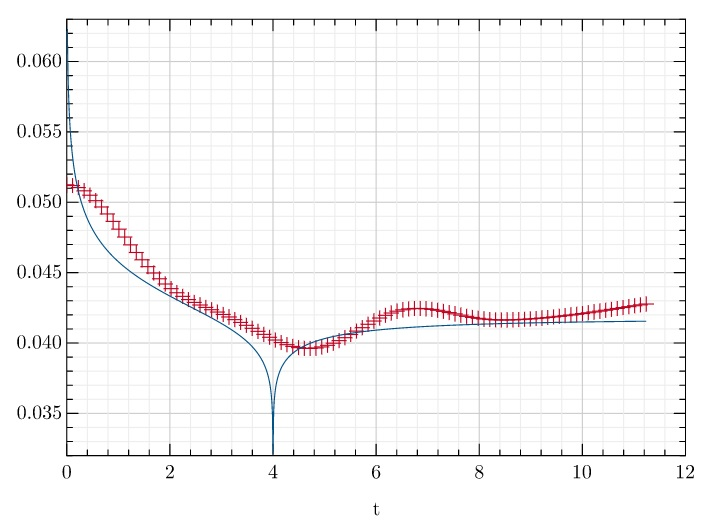
\includegraphics[width=0.9\linewidth]{XXZcor0.2}
      		\title{(a)$\Delta=0.2$,关联长度$l=8$}
      		\label{fig:27}
      	\end{minipage}
      	\begin{minipage}{0.49\linewidth}
      		\centering
      		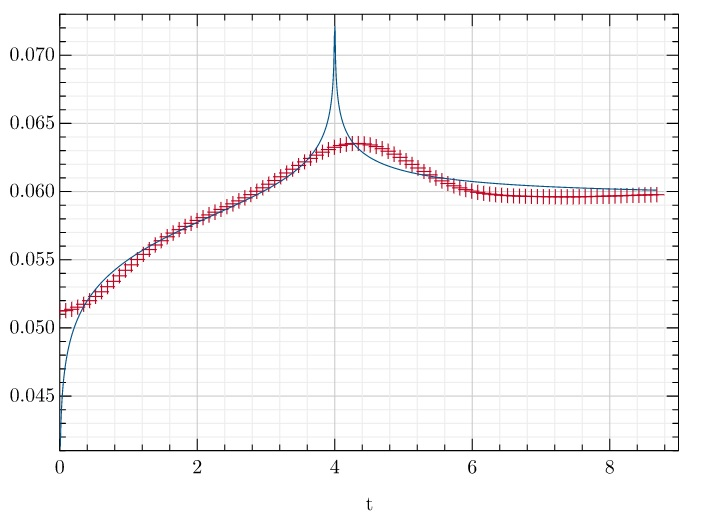
\includegraphics[width=0.9\linewidth]{XXZcor-0.2}
      		\title{(b)$\Delta=-0.2$,关联长度$l=8$}
      		\label{fig:28}
      	\end{minipage}
        
        \begin{minipage}{0.49\linewidth}
        	\centering
        	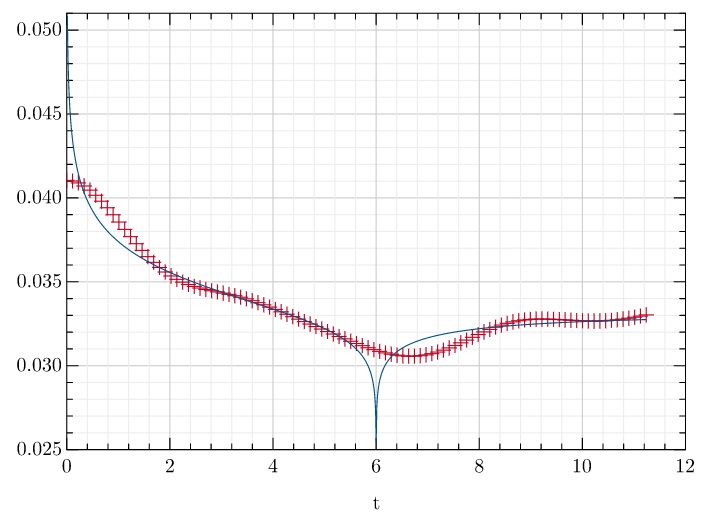
\includegraphics[width=0.9\linewidth]{XXZcor0.2l12}
        	\title{(a)$\Delta=0.2$,关联长度$l=12$}
        	\label{fig:27}
        \end{minipage}
        \begin{minipage}{0.49\linewidth}
        	\centering
        	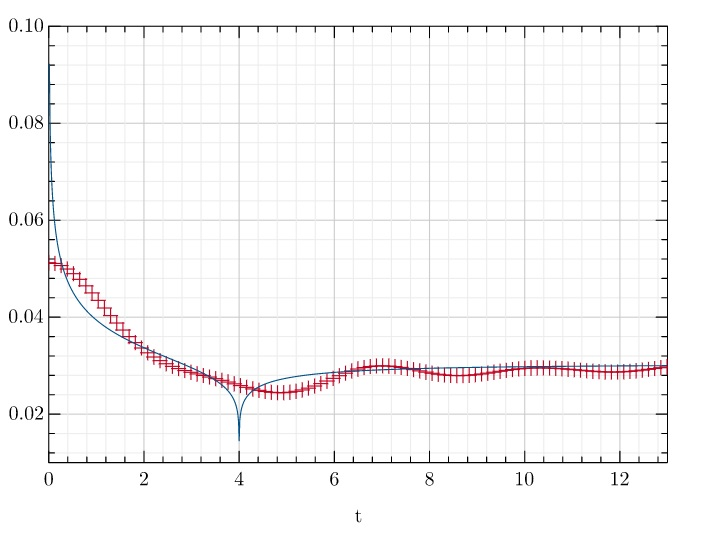
\includegraphics[width=0.9\linewidth]{XXZcor0.5}
        	\title{(b)$\Delta=0.5$,关联长度$l=8$}
        	\label{fig:28}
        \end{minipage}
      
      	\caption[9pt]{关联函数在quench后的时间演化,横轴为时间$t$,纵轴为关联函数$\langle S^x_{j}S^x_{j+l}\rangle$,蓝色实线为LL理论得到的解析解,红色线为DMRG+TDVP的数值解}
      \end{figure}
      
      \newpage
   {\centering\section{总结与展望}}


   \noindent{\heiti 总结}
   
   张量网络算法能够帮着我们更好地研究量子量子系统,它不仅可以得到哈密顿量的基态,也可以得到系统的时间演化。当我们有了波函数精确的数值描述,我们可以计算局域物理观测量,系统的纠缠,关联函数等等,这些性质可以帮助我们更好地理解量子多体系统。
   该研究方向被大家关注并不断有新的进展,自White在1992年提出DMRG算法,经过近20年的发展,张量网络算法不断丰富。从MPS到二维的PEPS,从DMRG到TEBD以及TDVP算法,包括现在张量网络和机器学习相结合\cite{carleo2017solving},诞生出了更有趣和高效的算法。
   
   本文在第一章介绍了最基础的用来描述一维量子系统的张量网络——矩阵乘积态(MPS),介绍了如何利用SVD分解构造MPS;MPS的纠缠熵和混合正交形式。第二详细章介绍了跟MPS相关的三种张量网络算法:DMRG、TEBD和TDVP,这三种算法既可以求解哈密顿量的基态,也可以研究系统的含时演化。第三章主要利用quantum quench的思想具体研究了一维横场伊辛模型和一维海森堡模型。本文数值求解了横场伊辛的z方向磁化$\langle\sigma_z\rangle$以及XXZ模型的自旋关联函数$\langle S_i^x S_j^x\rangle$,并将其与得到的解析表达式相比较。
   
   \noindent{\heiti 展望} 
   
   我们利用这些算法更深入地研究伊辛模型的跨相动力学演变,分析关联函数的演化形式。量化地探讨这些算法的相关误差并可以试图寻找优化形式以及研究纠缠熵在演化过程的变化形式,探讨其与误差的关系。另外我们也可以进一步从MPS到二维系统的研究,学习系统纠缠投影对态(Projected entangled-pairstate,PEPS),二维玻色子的MERA算法。随着张量网络领域的不断发展,我们对于量子多体系统的理解也会越来越清晰和深入。
   \newpage
      
   %\section{致谢}
   
   
   
   
   
   \bibliographystyle{IEEEtran}
   {\centering\bibliography{ref}}
   
\end{document}